\documentclass{beamer}[10pt]
\usepackage{listings}
\usepackage{xcolor}

\definecolor{codegreen}{rgb}{0,0.6,0}
\definecolor{codegray}{rgb}{0.5,0.5,0.5}
\definecolor{codepurple}{rgb}{0.58,0,0.82}
\definecolor{backcolour}{rgb}{0.95,0.95,0.92}

\lstdefinestyle{mystyle}{
    backgroundcolor=\color{backcolour},   
    commentstyle=\color{codegreen},
    keywordstyle=\color{magenta},
    numberstyle=\tiny\color{codegray},
    stringstyle=\color{codepurple},
    basicstyle=\ttfamily\footnotesize,
    breakatwhitespace=false,         
    breaklines=true,                 
    captionpos=b,                    
    keepspaces=true,                 
    numbers=left,                    
    numbersep=5pt,                  
    showspaces=false,                
    showstringspaces=false,
    showtabs=false,                  
    tabsize=2
}

\lstset{style=mystyle}


\usetheme{Madrid}
\setbeamertemplate{navigation symbols}{}
\title[DeAnonTor]{DeAnonimize TOR Network}
\subtitle[]{whit fingerprinting analisys}
\author[Paola Guarasci]{Paola Guarasci}
% \institute[Unical]{Università della Calabria}
\date[06/2022]{July 2022}

% Description of the specific BCP (BEST CURRENT PRACTICE)/CWE/CVE number, or in general, of the project topic.
% Whenever applicable, description of the technological context of the assigned BCP/CWE/CVE/General topic, including criticism, if any (e.g. show that a given BCP is outdated and why, etc.)
% Examples (for a CWE, an example can consist in a specific CVE)

\begin{document}
\frame{\titlepage}

\begin{frame}
  \frametitle{Descrizione del progetto}
  Il progetto prevede la deanonimizzazione di un utente TOR a partire dalle fingerprint dei siti web visitati. \\ In particolare e' possibile creare una correlazione tra le risorse e il traffico generato per la loro fruizione.

\end{frame}

\begin{frame}
  \frametitle{Aspetti tecnici}
\end{frame}

\begin{frame}
  \frametitle{Laboratorio}
  Il laboratio GNS3 realizzato per questo progetto conta un totale di 10 host Debian 11 emulati con QEMU, 3 router Cisco 7200 e 4 switch Cisco 3745.
  \begin{figure}
    \centering
    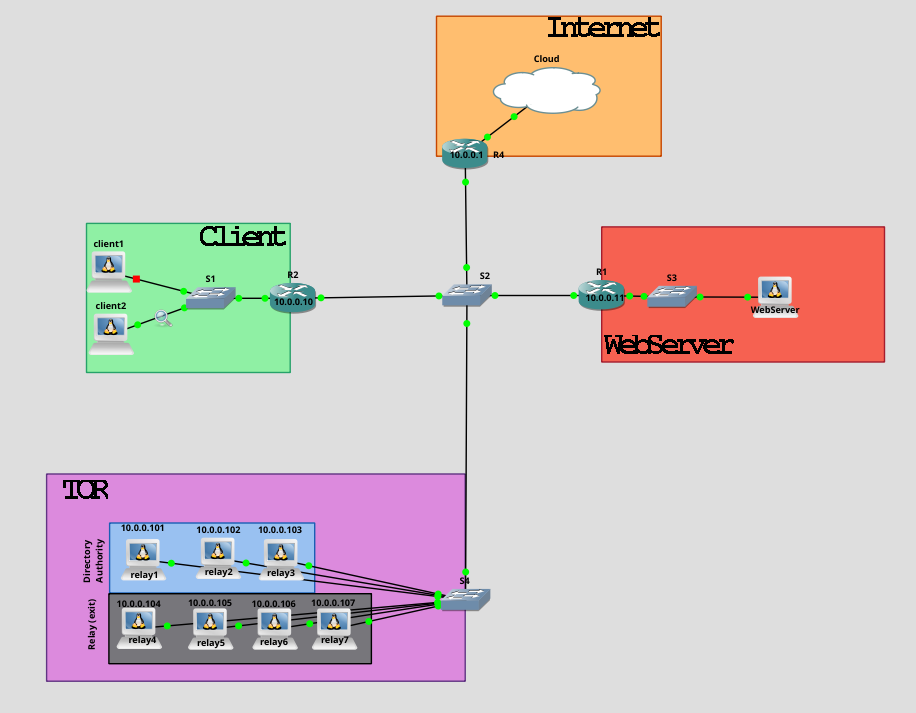
\includegraphics[width=0.60\textwidth]{../img/topology.png}
  \end{figure}

\end{frame}

\begin{frame}
  \frametitle{Rete Tor}
  La rete Tor e' stata creata partendo dalle configurazioni suggerite dal simulatore di reti Tor private (Chutney). Al suo interno la rete e' divisa in:
  \begin{itemize}
    \item 3 DA (Relay autoritativi)
    \item 4 Relay di uscita
  \end{itemize}
  Ognuno di questi host ha un accesso diretto alla rete interna del laboratorio, per simulare il piu' possibile il fatto che presumibilmente in un contesto reale questi server dispongono di un ip pubblico.
  La configurazione con 3 directory autority e' conseguenza di alcuni espreimenti in cui la rete non funzionava a dovere e ho poi compreso che le reti Tor necessitano di almeno 3 host auth/mid/exit per creare le rotte. In questi 3 elementi pero' ogni host non include se stesso. Questa configurazione 3+4 e' per me la configurazione minima funzionante.
\end{frame}


%% \begin{frame}
%%   \frametitle{Nuova slide}
%%
%% \end{frame}
%% 
%% 
%% \begin{frame}[fragile]
%%   \frametitle{Nuova slide Codice embeddato}
%% 
%%   \begin{lstlisting}[language=Python]
%%     import numpy as np
%%     def incmatrix(genl1,genl2):
%%         m = len(genl1)
%%         n = len(genl2)
%%         M = None #to become the incidence matrix
%%         VT = np.zeros((n*m,1), int)  #dummy variable        
%%     \end{lstlisting}
%% \end{frame}
%% 
%% 
%% \begin{frame}[fragile]
%%   \frametitle{Nuova slide Codice importato}
%%   \lstinputlisting[language=sh]{../src/creazioneLab/torNetwork/host/realy.sh}
%% \end{frame}
\end{document}